\problemname{Problem 7 - The Plot Thickens}

Professor Plum’s wife likes to paint, but Professor Plum is more of a digital kind of guy.  Imagine an $8$-by-$7$ canvas of zeroes as shown in Figure (a). Imagine plotting a $5$-by-$4$ rectangle of ones on it, with its top-left corner at $(2, 3)$, as shown in Figure (b).

\begin{figure}[h]
\begin{center}
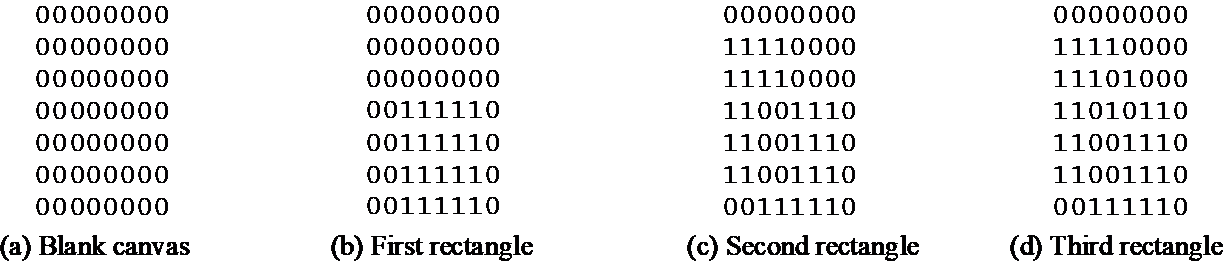
\includegraphics[width=0.9\textwidth]{problem7chart.png} 
\end{center}
\end{figure}

Imagine plotting a $4$-by-$5$ rectangle of ones on the current canvas, with its top-left corner at $(0, 1)$. However, whenever the rectangle overlaps any other rectangle, the pixels cancel each other out, as shown in Figure (c). Suppose further that we plot a $2$-by-$2$ rectangle at $(3, 2)$. The resulting canvas is shown in Figure (d). \\

After plotting a sequence of rectangles to a canvas in this manner, how many pixels are set to $1$?

\section*{Input}
The input consists of a number of cases followed by a line for each case. The first two numbers in each case’s line are the width and height of the canvas. The third number is the number of rectangles plotted. The remaining numbers describe each rectangle and therefore appear in groups of $4$. Within a group, the first two numbers are the $xy$-coordinates of a rectangle’s top-left corner, and the second two are the rectangle’s dimensions.

\section*{Output}
For each case, print a case label and the number of 1-pixels in the canvas after all plotting. For the example input, the output is: